\documentclass[11pt]{article}
\usepackage{amsfonts}%For Maths fonts.
\usepackage{amssymb}%For math symbols.
\usepackage{amsmath}%For the math.
\usepackage{graphicx}%For the image.
\graphicspath{ ./} 
\usepackage{tikz}
\usepackage{float}
\usepackage{hyperref} 
\usepackage{listings}
\usepackage{color}
\usepackage{csvsimple}

\definecolor{dkgreen}{rgb}{0,0.6,0}
\definecolor{gray}{rgb}{0.5,0.5,0.5}
\definecolor{mauve}{rgb}{0.58,0,0.82}

\lstset{frame=tb,
	language=python,
	aboveskip=3mm,
	belowskip=3mm,
	showstringspaces=false,
	columns=flexible,
	basicstyle={\small\ttfamily},
	numbers=none,
	numberstyle=\tiny\color{gray},
	keywordstyle=\color{blue},
	commentstyle=\color{dkgreen},
	stringstyle=\color{mauve},
	breaklines=true,
	breakatwhitespace=true,
	tabsize=3
}

\usetikzlibrary{shapes.geometric, arrows}%For the borders and shapes.
\begin{document}
	\begin{titlepage}
		\begin{flushleft}
			
			\bf CS7.301
			\hfill
			\bfseries 13$^{th}$ Feb, 2020
		\end{flushleft}
		\begin{center}
			\line(1,0){300}\\
			[5mm]
			\huge{\bfseries MDL Assignment-1}\\
			\line(1,0){300}\\
			[12cm]
		\end{center}
		\begin{flushright}
			{
				\line(1,0){270}\\
				\large  Vikrant Dewangan, Roll No.- 2018111024\\  Mohammad Nomaan Qureshi,
				Roll No.- 2018111027
				\line(1,0){270}\\
			}
		\end{flushright}
	\end{titlepage}
	\newpage
	\tableofcontents
	\newpage
	
	\section{Question 1}
	\subsection{Problem Statement}
	Given a data set of 5000 data points, train a linear classifier and calculate
	the bias and variance of the trained model for different functions upto degree
	9, always ensuring a 90:10 split between training and testing data. 
	\subsection{Algorithm Implementation}
	The following steps are followed to obtain the final set of values - 
	\begin{enumerate}
		\item First the given data in pickle format is loaded and uniformly shuffled.
		\begin{lstlisting}
		#=================================================================#
		# Loading the Data file #
		#=================================================================#
		file = open('Q1_data/data.pkl', 'rb')
		data = pickle.load(file)
		print("Loaded Data Successfully!!!")
		#=================================================================#
		
		
		#=================================================================#
		# Resampling Data #
		# First randomly Shuffle data into 10 equal parts and then divide them into 10
		equal parts.
		#=================================================================#
		np.random.shuffle(data)
		\end{lstlisting}	
		\item Preparing Train and Test data set
		\begin{lstlisting}
		test = data[:len(data)//10]
		train = data[len(data)//10:]
		
		random.shuffle(train)
		train_y = np.asarray([[i[1]] for i in train])
		test_y  = np.asarray([[i[1]] for i in test])
		
		train_x = np.asarray([np.asarray([i[0]**j for j in range(1, 10)]) for i in
		train])
		test_x = np.asarray([np.asarray([i[0]**j for j in range(1, 10)]) for i in
		test])
		
		\end{lstlisting}
		As specified in the problem statement, the first 10 parts of data are prepared
		as training and the last part as test data set. After which, the data is
		structured in a proper format using numpy arrays.
		\item Training 10 different models using 10 different functions
		\begin{lstlisting}
		coef = []			# Coefficient Obtained by Regression #
		intercept = []		# Intercept Obtained by Regression   #
		err, var, bas = [], [], []
		for j in range(1, 10):
		prediction = np.zeros((len(test_x), 1))
		pred_array = []
		variance = 0
		mse = []
		for i in range(10) :
		if j == 1 :
		fit_intercept = False
		else :
		fit_intercept = True
		reg = LinearRegression(fit_intercept=fit_intercept, normalize =
		True).fit(train_x[i*len(train_x)//10:(i+1)*len(train_x)//10, :j],
		train_y[i*len(train_x)//10:(i+1)*len(train_x)//10])
		coef.append(reg.coef_)
		pred = reg.predict(test_x[:,:j])
		pred_array.append(pred)
		prediction = prediction + pred
		
		\end{lstlisting}
		The function \textbf{LinearRegression} is used to fit the model and the
		corresponding part of the [train\_x,train\_y] array is given as parameters to
		the function.
		The array \textit{coef} signifies the coefficients obtained in the linear
		regression fit every time it is called. Thus, by appending it to the array, each
		time, a function of order \textit{j} is used to train the model.
		
		\item Calculating mean variance and bias for each function
		\begin{lstlisting}
		pred_array = np.asarray(pred_array)
		prediction = prediction/10
		diff = pred_array - prediction
		bias = np.mean((prediction - test_y))**2
		variance = np.mean(diff**2)
		err.append(np.mean(mse))
		var.append(variance)
		bas.append(bias)
		\end{lstlisting}
		Here are what all of the variables signify - 
		\begin{itemize}
			\item \textit{pred} represents the predicted value \textit{\^{f}(x)}
			\item \textit{prediction} is the sum of all predictions done by the model.
			Used to calculate
			$E\big[\textit{\^{f}(x)}\big]$
			\begin{align*}
			E\big[\textit{\^{f}(x)}\big] &= \frac{\sum_{j=1}^{10}\textit{\^{f}(x)}}{10}
			\end{align*}
			\item \textit{bias} is calculated as mean of \textit{prediction} and
			\textit{test\_y} arrays.
			In other words,
			\begin{align*}
			Bias^2 &= \bigg(E\bigg[E\big[\textit{\^{f}(x)}\big]-f(x)\bigg]\bigg)^2 \\
			&= \bigg(E\big[\textit{\^{f}(x)}\big]-f(x)\bigg)^2
			\end{align*}
			\item \textit{variance} is calculated as the mean of prediction values
			\textit{\^{f}(x)} and average prediction value $E\big[\textit{\^{f}(x)}\big]$
			\begin{align*}
			Variance &=
			E\bigg[\big(\textit{\^{f}(x)}-E\big[\textit{\^{f}(x)}\big]\big)^2\bigg]
			\end{align*}
			\item \textit{mse} is calculated by the function
			\textit{mean\_squared\_error} function and can be given by the formula
			\begin{align*}
			M.S.E &= E\big[\big(\textit{\^{f}(x)}-f(x)\big)^2\big] + \sigma^{2}
			\end{align*}
			where $\sigma^{2}$ is the variance of the noise with mean($\mu$) = 0
		\end{itemize}
	\end{enumerate}
	Thus, for each polynomial, mean bias and variance are calculated and tabulated. 
	
	\subsection{Results}
	The following is the result of the data shuffling. 
	\begin{center}
		\hspace{-1.5cm}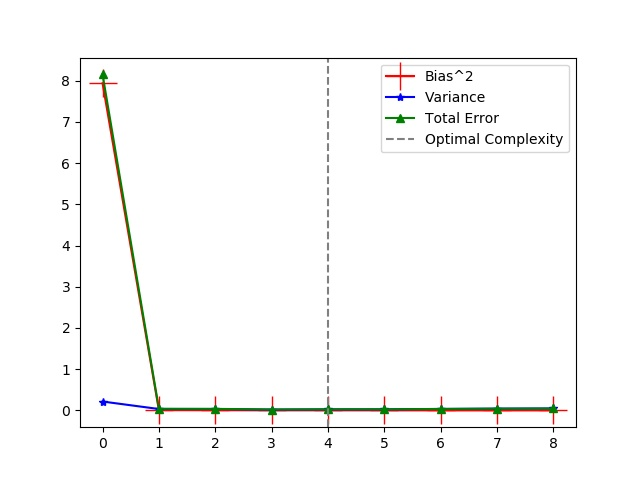
\includegraphics[scale=0.8]{../q1.jpg}		
	\end{center}
	In tabular version - 
	%	\csvreader[]{q1.csv
\begin{center}
	\begin{tabular}{|l|l|l|l|}
		\hline
		\textbf{Model Complexity} & \textbf{Bias}     & \textbf{Variance} & \textbf{Total Error} \\ \hline
		1                         & 5.46952589256     & 0.205035064745    & 5.67456095731        \\ \hline
		2                         & 0.00946157459989  & 0.0311687828902   & 0.0406303574901      \\ \hline
		3                         & 0.00132121430958  & 0.0637597311871   & 0.0650809454967      \\ \hline
		4                         & 0.00668651415434  & 0.0335039036798   & 0.0401904178342      \\ \hline
		5                         & 0.00335006723856  & 0.0362704492444   & 0.039620516483       \\ \hline
		6                         & 0.000368344916076 & 0.0418653802428   & 0.0422337251589      \\ \hline
		7                         & 0.000666255490301 & 0.0538722377555   & 0.0545384932458      \\ \hline
		8                         & 0.000572732337839 & 0.0649197944417   & 0.0654925267795      \\ \hline
		9                         & 0.000691939933171 & 0.0624076730169   & 0.06309961295        \\ \hline
	\end{tabular}
\end{center}
		\textbf{Note} that the \textit{pred\_array} is an array containing the values and thus the bias and variance are already calculated in a \textbf{\textit{vectorized}} manner on numpy arrays.
	\subsection{Inferences}
		Following can be inferred from the data - 
	\begin{itemize}
		\item Initially, bias seems to be very high for a naively complex model (i = 1). It signifies that the trained model seems to underfit with the test data as well as the trained data. As we could see the plot below, the model is not only failing on data both training and testing. The variance seems to be low initially as it consistently. This is an example of \textbf{Underfit} model.
			\begin{center}
		\hspace{-1.5cm}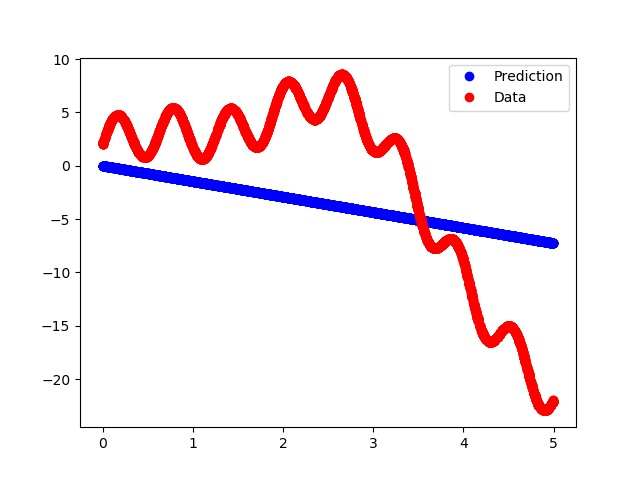
\includegraphics[scale=0.8]{../q1fig1.jpg}
	\end{center}
		\item As we increase the complexity, bias drops drastically and the model is able to almost accurately predict the trend. However, due to increase in parameters, a small change in test data results in very high change in the predictive model. For us, we achieve the optimal complexity at order of 4. 
			\begin{center}
		\hspace{-1.5cm}	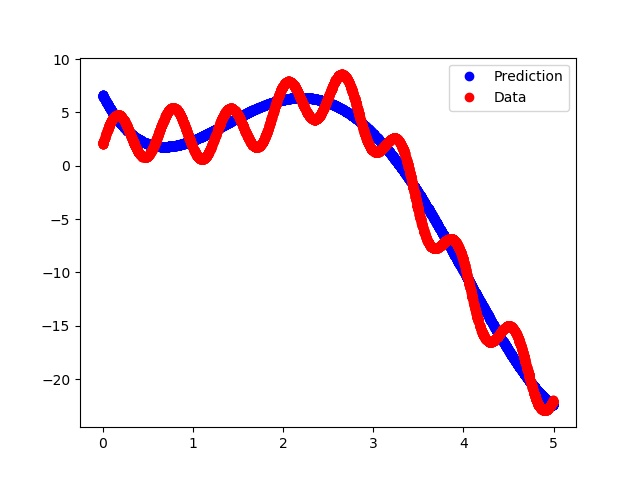
\includegraphics[scale=0.8]{../q1fig4.jpg}
	\end{center}
		\item Further ,if we increase the complexity more, we get a model highly \textbf{Overfit}. In that, it is involving a very high variance. Any small changes in the test data results in the parameters getting severely changed. Although the model involves very low bias, we don't choose it because of the high total error present in the model due to high variance.
				\begin{center}
		\hspace{-1.5cm}	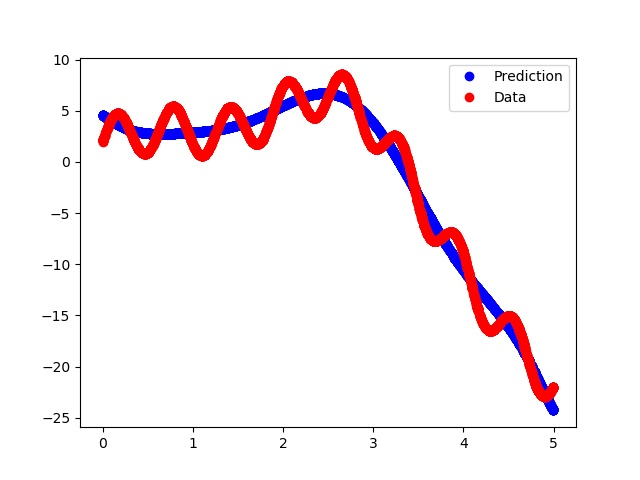
\includegraphics[scale=0.8]{../q1fig9.jpg}
		\end{center}
	\end{itemize}

	\section{Question 2}
	\subsection{Problem Statement}
	Given 20 subsets of training data containing 400 samples each, train 20 models
	on each subset of data and observe the bias and variance on testing data.
	Comment on the fit of the model by plotting the bias-variance graph. 
	\subsection{Algorithm Implementation}
	\begin{enumerate}
		\item Loading the data file
		\begin{lstlisting}
		#=============================================================================#
		# Loading the Data file #
		#=============================================================================#
		file = open('Q2_data/Fx_test.pkl', 'rb')
		test_y = pickle.load(file)
		file.close()
		file = open('Q2_data/X_test.pkl', 'rb')
		test_x = pickle.load(file)
		file = open('Q2_data/X_train.pkl', 'rb')
		train_x = pickle.load(file)
		file = open('Q2_data/Y_train.pkl', 'rb')
		train_y = pickle.load(file)
		print("Loaded Data Successfully!!!")
		#=============================================================================#
		\end{lstlisting}
		\item Training a polynomial model on given data.
		\begin{lstlisting}
		for i in range(10) :
			prediction = np.zeros((80, 1))
			pred_array = []
			variance = 0
			mse = []
			for j in range(20) :
				poly = PolynomialFeatures(degree = i)
				subTr_x = np.reshape(train_x[j], (400, 1))
				subTr_y = train_y[j]
				subTr_x = poly.fit_transform(subTr_x)
				reg = LinearRegression().fit(subTr_x, subTr_y)
				subTs_x = test_x
				subTs_x = poly.fit_transform(subTs_x)
				pred = np.reshape(reg.predict(subTs_x), (80, 1))
				pred_array.append(pred)
				prediction = prediction + pred
		\end{lstlisting}
		We have used the \textbf{PolynomialFeatures()} function which generates a feature matrix consisting of all polynomial combinations of the features with degree less or equal to specified degree. In each iteration, \textit{subTr\_x} is train the model via the \textbf{LinearRegression().fit()} function. After this, the model is then fitted onto the test data using the \textbf{poly.fit\_transform()} function. 
		
		\item Finding the mean variance and bias.
		\begin{lstlisting}
			pred_array = np.asarray(pred_array)
			prediction = prediction/20
			diff = pred_array - prediction
			bias = (np.mean((prediction - test_y))**2)
			variance = np.mean(diff**2)
		\end{lstlisting}
		Bias$^2$ and variance are found out as per the formulae mentioned above. 
		
		\textbf{Note} that the \textit{pred\_array} is an array containing the values and thus the bias and variance are already calculated in a \textbf{\textit{vectorized}} manner on numpy arrays.
	\end{enumerate}
	\subsection{Results}
	Here is the scatter plot of the given data - 
	\begin{center}
			\hspace{-1.5cm}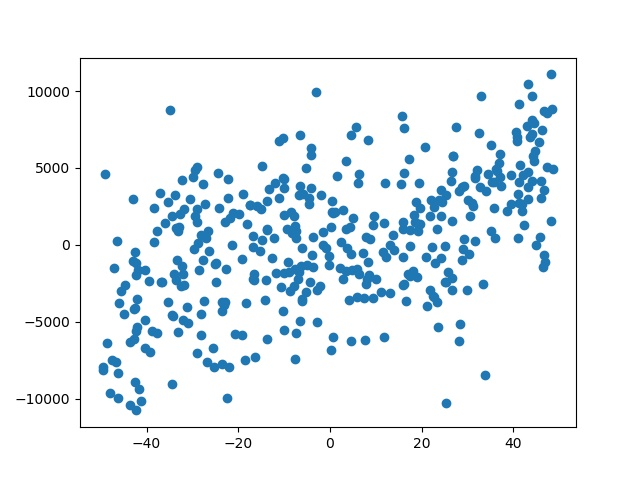
\includegraphics[scale=0.8]{../q2scatter.jpg}
	\end{center}
	\begin{center}
		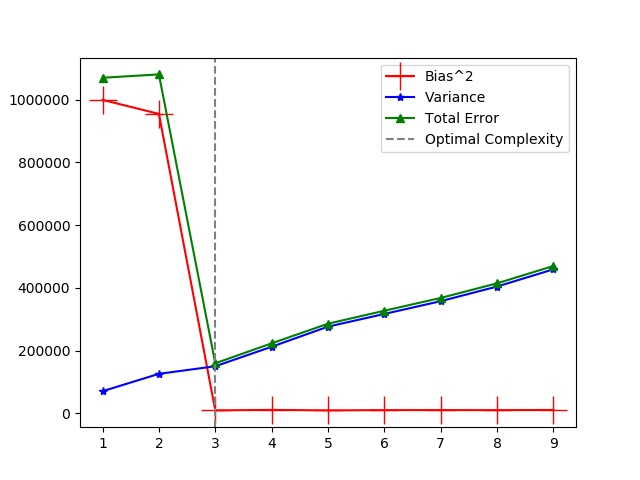
\includegraphics{../q2.jpg}
	\end{center}
	Here is the tabulated version of the following data - 
	\begin{center}
		\begin{tabular}{|l|l|l|l|}
			\hline
			\textbf{Model Complexity} & \textbf{Bias} & \textbf{Variance} & \textbf{Total Error} \\ \hline
			1                         & 999228.396872 & 70545.4891458     & 1069773.88602        \\ \hline
			2                         & 954619.273794 & 125870.855549     & 1080490.12934        \\ \hline
			3                         & 9389.73011679 & 150073.739546     & 159463.469663        \\ \hline
			4                         & 10907.348134  & 212235.708326     & 223143.05646         \\ \hline
			5                         & 9339.19428314 & 276388.480184     & 285727.674467        \\ \hline
			6                         & 10248.586398  & 316863.497736     & 327112.084133        \\ \hline
			7                         & 10335.2794411 & 357511.103478     & 367846.382919        \\ \hline
			8                         & 10149.4951806 & 404289.174765     & 414438.669946        \\ \hline
			9                         & 10715.8079055 & 459113.935504     & 469829.74341         \\ \hline
		\end{tabular}
	\end{center}

	\subsection{Inferences}
	Following can be inferred from the data - 
	\begin{itemize}
		\item Initially, bias seems to be very high for a naively complex model (i = 1). It signifies that the trained model seems to underfit with the test data as well as the trained data. As we could see the plot below, the model is not only failing on data both training and testing. The variance seems to be low initially as it consistently. This is an example of \textbf{Underfit} model.
		\begin{center}
		\hspace{-1.5cm}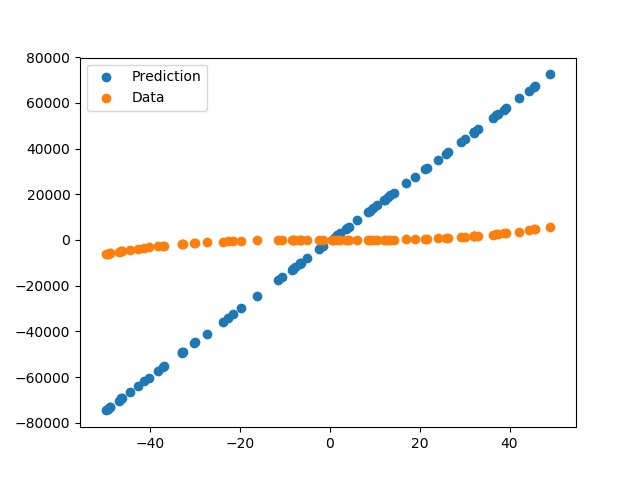
\includegraphics[scale=0.8]{../q2fig1.jpg}
		\end{center}
		\item As we increase the complexity, bias drops drastically and the model is able to almost accurately predict the trend. However, due to increase in parameters, a small change in test data results in very high change in the predictive model. For us, we achieve the optimal complexity at order of 3.
		\begin{center}
	\hspace{-1.5cm}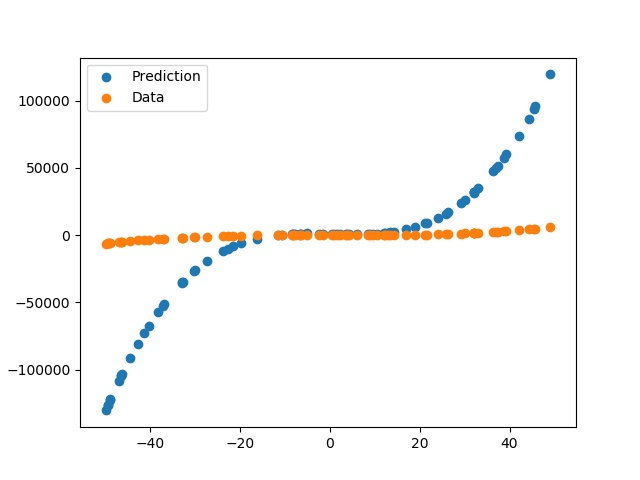
\includegraphics[scale=0.8]{../q2fig3.jpg}
\end{center}
		\item Further ,if we increase the complexity more, we get a model highly \textbf{Overfit}. In that, it is involving a very high variance. Any small changes in the test data results in the parameters getting severely changed. Although the model involves very low bias, we don't choose it because of the high total error present in the model due to high variance.
		\begin{center}
	\hspace{-1.5cm}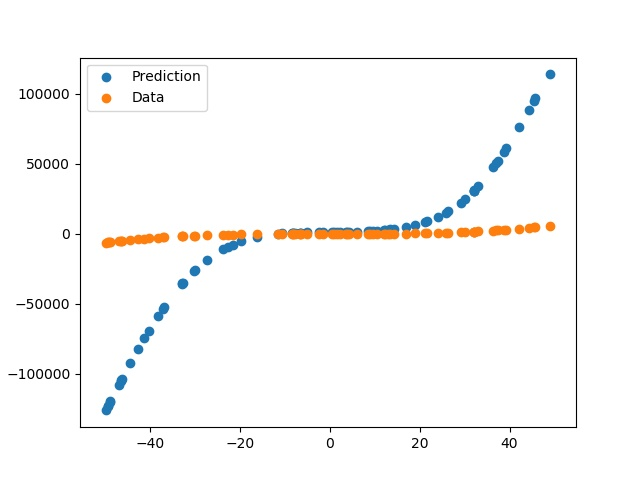
\includegraphics[scale=0.8]{../q2fig9.jpg}
\end{center}
		\item Upon looking at the plot, we offer to comment the following on the data - 
		\begin{enumerate}
			\item The data has very high variance, in that it requires a model of complexity 3 to be fit.
			\item Also, the data is very noisy, since at particular points we obtain multiple values. 
		\end{enumerate}
		
	\end{itemize}
\end{document}

